\subsection{Step Response Characterisation}

The first step to calculating $T$, $r$, and $n$ is to  understand  how the order
$n$ influences the shape of the transfer function's step response.

It is important to realise that no matter how a step response function is scaled
or  offset  (defined  by the parameters $K_s$ for amplitude, $T$ for time scale,
$x_0$ and $y_0$ for offset) the actual \textit{shape}  always  remains the same.
Thus, only its shape tells us something about its complexity.

Therein  lies  the  key. A method  needs  to  be  devised  for  determining  how
``simple''  or  how ``complex'' a step response is -- independent of  scale  and
offset -- before  it  is possible to start modelling and fitting a system to it.

This ``complexity'' is \textbf{directly related}  to  the  required order $n$ of
the transfer function.


\subsubsection*{P. Hudzovic's Approach}

P. Hudzovic proposed the following method (see figure \ref{fig:tu_tg}):

\begin{itemize}
    \item
Find  the  point  of  inflection of the step function. This  typically  involves
calculating the derivative and searching for a maximum.
    \item
Place a tangent  in  said  point and find the intersections with the minimum and
maximum horizontal lines.
    \item
The distance between the two intersections  is  referred  to  as  $T_g$, and the
distance between  the minimum intersection point and the beginning of the signal
is referred to as $T_u$.
\end{itemize}

The ``complexity'' of the  step  response  is  defined by the ratio of $T_u$ and
$T_g$ and is written as:

\begin{equation}
    \textrm{plant}_{Tu/Tg} = \frac{T_u}{T_g}
    \label{eq:tu_tg}
\end{equation}


\subsubsection*{L. Sani's Approach}

L.  Sani  proposed   a  different  method  (see  figure  \ref{fig:t10_t50_t90}):
Determine the  times  $t_{10}$,  $t_{50}$ and $t_{90}$ required for reaching the
values   at    \SI{10}{\percent},    \SI{50}{\percent}    and   \SI{90}{percent}
respectively.

The   ``complexity''   of  the  step  response  is  defined  by  the  ratio   of
$t_{90}-t_{10}$   and   $t_{50}$,   otherwise   referred   to   as    $\lambda$:

\begin{equation}
    \textrm{plant}_{\lambda} = \frac{t_{90}-t_{10}}{t_{50}}
    \label{eq:t10_t50_t90}
\end{equation}


\subsubsection*{Short Visual Explanation}

Visually, one can see how decreasing $T_g$ in figure \ref{fig:tu_tg}  causes the
step  response  to become steeper (i.e. it becomes  more  ``complex''  and  thus
requires  a  higher  order  $n$)  and the value of $\textrm{plant}_{T_u/T_g}$ in
equation  \ref{eq:tu_tg}  increases.   Similarly,   decreasing   the  difference
$t_{90}-t_{10}$ in figure \ref{fig:t10_t50_t90} also causes the step response to
become  steeper  and causes the value of  $\textrm{plant}_{\lambda}$  increases.

On the other hand, one can  also see how increasing $T_u$ and $t_{50}$ increases
the delay  time  of  the  step  response,  which  similarly  leads  to  a higher
``complexity'', and thus, a higher order $n$.

How $n$ is calculated will become clear in the next section.

\begin{figure}[t]
    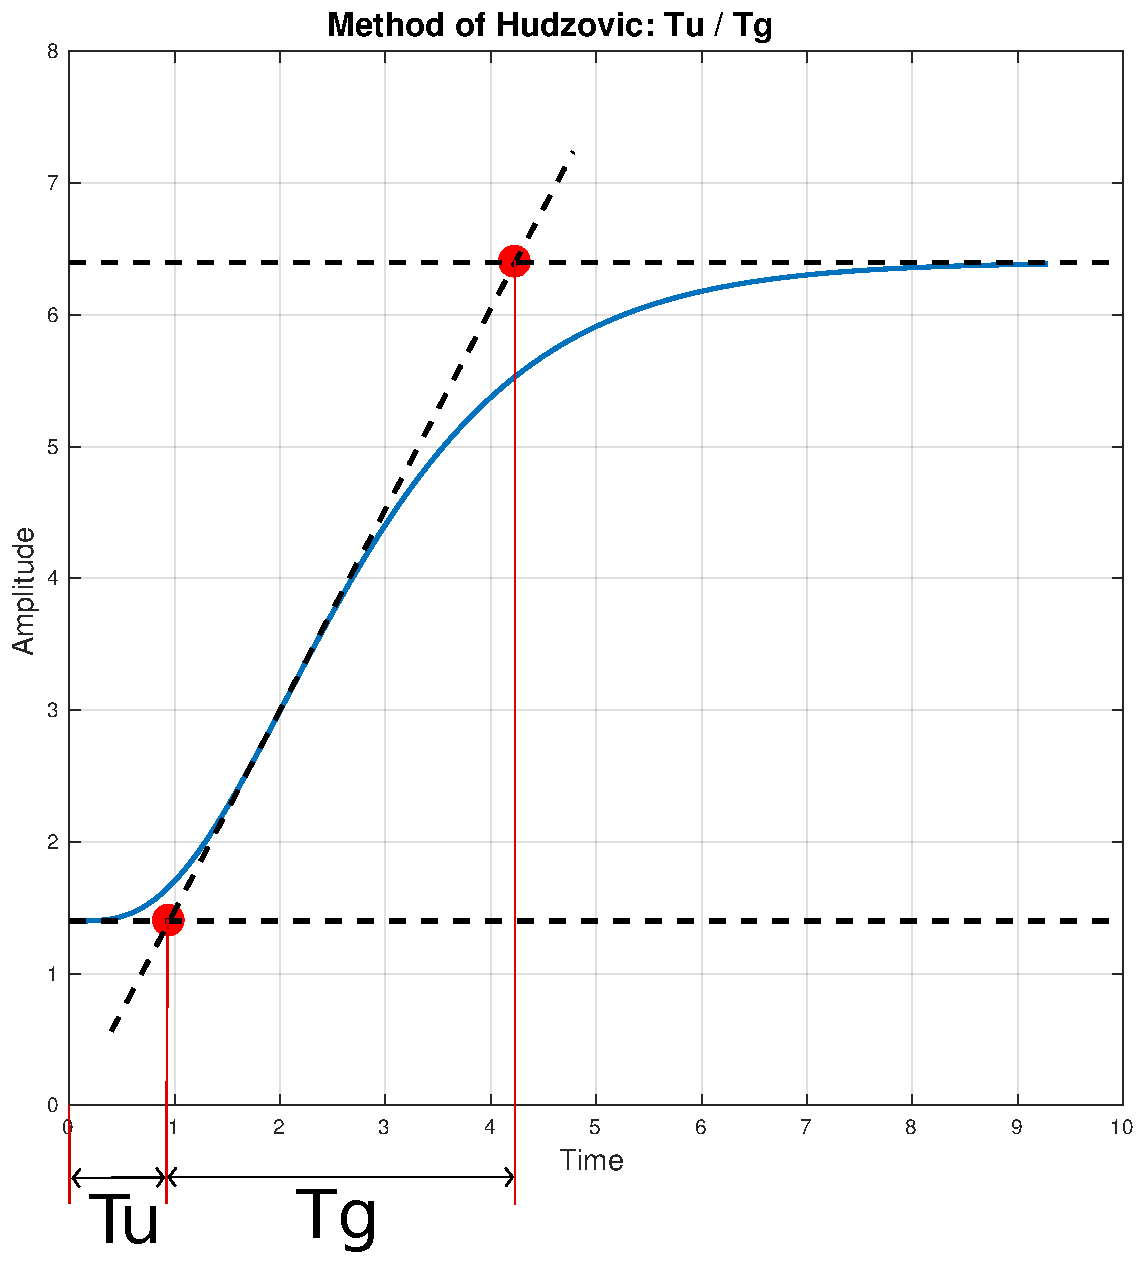
\includegraphics[width=\linewidth]{images/step_response_tu_tg}
    \caption{Method of P. Hudzovic, determine Tu and Tg}
    \label{fig:tu_tg}
\end{figure}
\begin{figure}[t]
    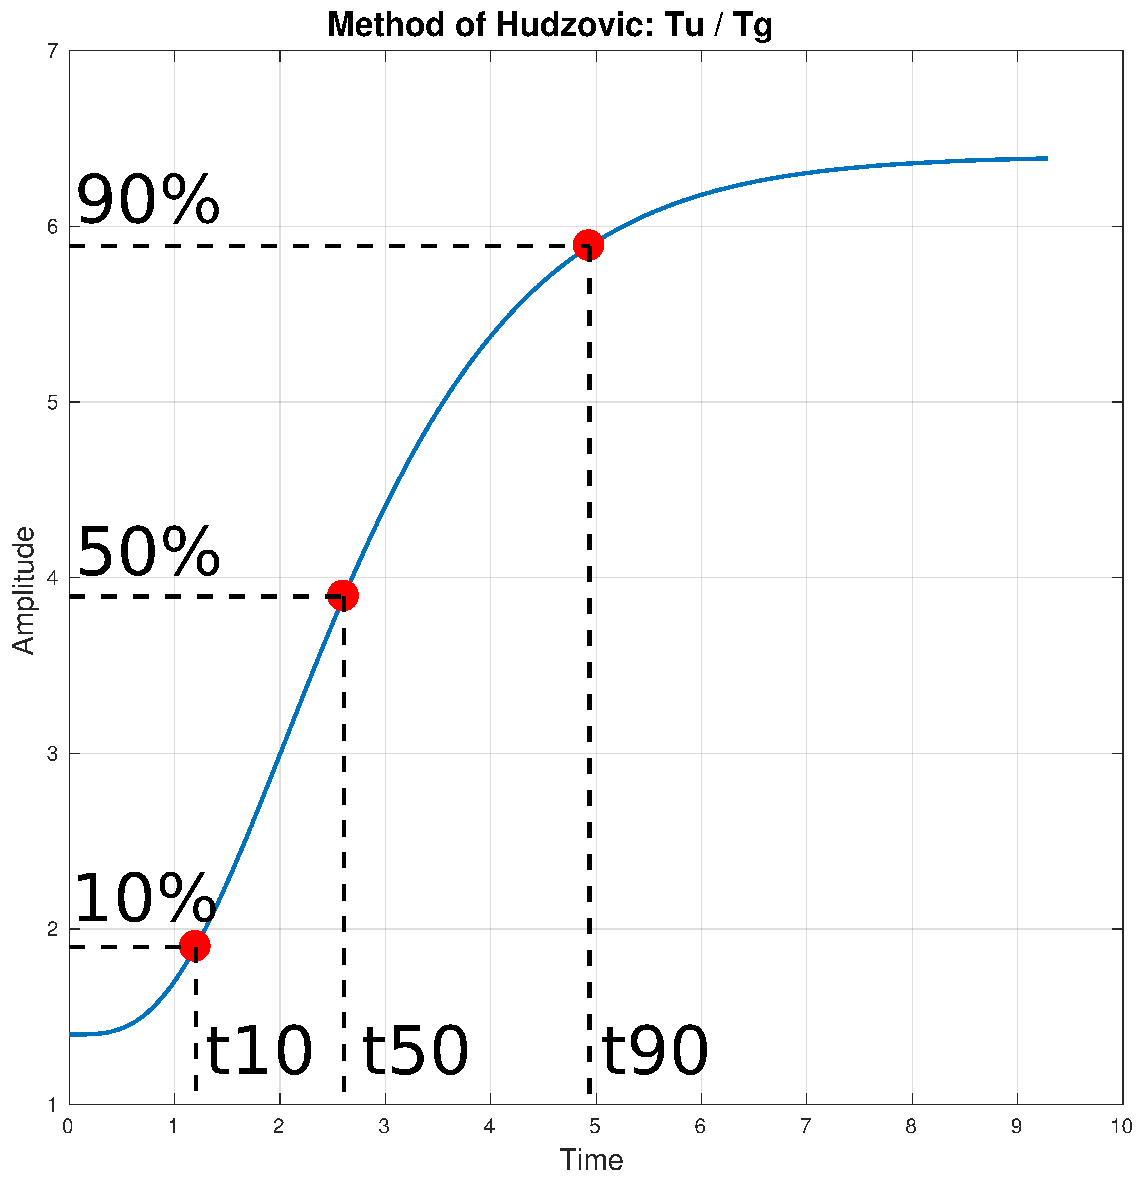
\includegraphics[width=\linewidth]{images/step_response_t10_t50_t90}
    \caption{Method of L. Sani, determine t10, t50 and t90}
    \label{fig:t10_t50_t90}
\end{figure}

